% EdgeLM -- initial paper draft
% Springer LNCS class (llncs). Compile: pdflatex -> bibtex -> pdflatex x2
% Required files in the same Overleaf project:
%   llncs.cls, splncs04.bst (both provided by Springer), references.bib
%
\documentclass[runningheads]{llncs}
%
\usepackage[T1]{fontenc}
\usepackage{graphicx}
\usepackage{booktabs}
\usepackage{amsmath}
\usepackage{amssymb}
\usepackage{tikz}
\usetikzlibrary{arrows.meta,positioning}
%
% To display URLs in blue roman per Springer's eBook style, uncomment:
%\usepackage{color}
%\renewcommand\UrlFont{\color{blue}\rmfamily}
%\urlstyle{rm}
%
\begin{document}
%
\title{EdgeLM: A Capability-First Benchmark for Sub-4B Language Models on Consumer Hardware}
%
\titlerunning{EdgeLM: A Capability-First Benchmark for Sub-4B LLMs}
%
\author{First Author\inst{1}\orcidID{0000-0000-0000-0000} \and
Second Author\inst{2}\orcidID{0000-0000-0000-0000}}
%
\authorrunning{F. Author et al.}
%
\institute{First Institution, City, Country \\
\email{first.author@example.edu} \and
Second Institution, City, Country \\
\email{second.author@example.edu}}
%
\maketitle
%
\begin{abstract}
The frontier of on-device language modelling has converged on the sub-4B
parameter regime: the most capable on-device production models now activate
only one to four billion parameters per prompt, and recent evidence suggests
that verifiable reasoning compresses into a compact parametric core even as
broad knowledge does not. Existing edge-LLM benchmarks, however, optimize
almost exclusively for systems metrics---throughput, energy, and memory---and
reduce task quality to a single multiple-choice accuracy number. We introduce
\emph{EdgeLM}, a capability-first benchmark that decomposes generative ability
at the sub-4B scale into six task families: context retention under
conversational load, cross-domain summarization, open-book comprehension,
structured-output compliance, constrained creative generation, and
execution-verified code generation across Python and a low-resource language.
EdgeLM evaluates fifteen openly available sub-4B models spanning several base
families, including two clean base-to-finetune pairs that isolate post-training
effects on a fixed backbone. All evaluation stimuli are human-authored rather
than model-generated, and scoring is matched to each task: deterministic
parsers and code execution where outputs are objectively checkable, and
calibrated judging elsewhere. We frame the benchmark as a direct test of the
reasoning--knowledge decoupling hypothesis at this scale, predicting that
compact models remain competitive on reasoning- and format-bound tasks while
degrading on knowledge-intensive comprehension and summarization. We describe
the benchmark design, the model roster, and the evaluation protocol in detail.

\keywords{Edge AI \and Small Language Models \and Benchmarking \and On-Device Inference \and Model Evaluation \and Reasoning}
\end{abstract}
%
\section{Introduction}

Large language models are increasingly deployed on edge and consumer
hardware, where local inference reduces latency, preserves privacy, and removes
dependence on cloud infrastructure. The binding constraint in this setting is
not raw compute but memory bandwidth: generative inference is governed by how
many parameters must be resident and active per forward pass. As a consequence,
the practical target for on-device deployment has settled on the sub-4B
\emph{active}-parameter regime. Notably, the most capable current on-device
production models adopt sparse architectures that activate only one to four
billion parameters per request~\cite{appleafm3}, while the previous generation
shipped a dense ${\sim}3$B model preferred by human graders over substantially
larger 7--8B baselines~\cite{appleafm2025}.

Parallel to this hardware convergence, a line of work on small reasoning models
argues that capability and scale are only partially coupled. Verifiable
reasoning---mathematics, coding, and constraint satisfaction, where answers can
be checked---appears to be ``parameter-dense'' and compressible into a small
reusable core, whereas open-domain knowledge is ``parameter-expansive'' and
scales with size~\cite{vibethinker2026}. A 3B model can thus reach
first-tier performance on verifiable benchmarks while remaining far behind on
knowledge-heavy evaluations. This decoupling has direct implications for how
sub-4B models should be evaluated, yet it has not been tested through a
controlled, multi-capability benchmark at this scale.

Existing edge-LLM benchmarks are ill-suited to the question. They are
predominantly systems-oriented, pairing a single aggregate accuracy figure with
device-level measurements of throughput, energy, and
latency~\cite{edgebench2026,leaf2026,rooflinebench2026}. Such benchmarks
establish the accuracy--efficiency trade-off but treat ``accuracy'' as a thin,
undifferentiated quantity, typically drawn from a multiple-choice suite that is
vulnerable to contamination and benchmark-specific optimization. No existing
benchmark decomposes \emph{generative} capability at the sub-4B scale into
distinct, separately scored task families.

We address this gap with \emph{EdgeLM}. Our contributions are:

\begin{enumerate}
\item A \textbf{capability-first benchmark} for sub-4B language models,
organized as a gradient of six task families that each presuppose the previous:
context retention, summarization, comprehension, structured output, creative
generation, and code generation (Section~\ref{sec:benchmark}).
\item A \textbf{controlled model roster} of fifteen openly available sub-4B
models spanning several base families, including two clean base-to-finetune
pairs and one within-family post-training pair that isolate the effect of
post-training on a fixed backbone (Section~\ref{sec:models}).
\item A \textbf{human-authored, contamination-resistant evaluation protocol}
with task-matched scoring---deterministic parsers and sandboxed code execution
where outputs are objectively checkable, and calibrated judging elsewhere---%
together with a reproducible reference harness that applies each model's correct
chat template, splits reasoning traces from final answers, and logs the
truncated-reasoning and context-overflow states needed to interpret small-model
failures (Section~\ref{sec:method} and Section~\ref{sec:setup}).
\item A framing of the benchmark as a \textbf{direct test of the
reasoning--knowledge decoupling hypothesis} at the sub-4B scale, with concrete
per-category predictions (Section~\ref{sec:discussion}).
\end{enumerate}

\section{Related Work}
\label{sec:related}

\subsubsection{Edge and on-device LLM benchmarking.}
The closest prior work benchmarks compact open-weight models on constrained
hardware, pairing generation-based accuracy with on-device power
measurements~\cite{edgebench2026}, or scoring deployments across energy,
speed, and semantic-accuracy pillars~\cite{leaf2026}. Hardware-aware analyses
formalize the ``memory wall'' that makes generative inference
bandwidth-bound rather than compute-bound~\cite{rooflinebench2026}. Surveys
catalogue the small-language-model and on-device inference
landscape~\cite{slmsurvey2024,edgeintelligence2026,ondeviceai2025}. These
efforts are systems-first; their task-quality signal is a single accuracy
number. EdgeLM is complementary: it is capability-first, decomposing generative
ability into separately scored families while remaining compatible with a
lightweight systems axis.

\subsubsection{Small reasoning models and the decoupling hypothesis.}
Distilling the reasoning traces of a large teacher into a small student has been
shown to outperform reinforcement learning applied directly to the small
model~\cite{deepseekr1}; reinforcement-learning fine-tunes of such distilled
1.5B models then surpass earlier frontier reasoning systems on competition
mathematics~\cite{deepscaler2025,fastcurl2025}. The decoupling hypothesis makes
the pattern explicit: compact models can match much larger systems on verifiable
reasoning while lagging on knowledge-intensive
benchmarks~\cite{vibethinker2026}. EdgeLM operationalizes this as a testable
prediction across its six categories.

\subsubsection{Task-specific evaluation lineages.}
Each EdgeLM category extends an established evaluation line. Long-context
behaviour is studied through synthetic retrieval and tracing
benchmarks~\cite{ruler2024} and the positional ``lost-in-the-middle''
effect~\cite{lostmiddle2023}, with later work showing that hard, semantically
related distractors understate difficulty relative to random
ones~\cite{lcrag2025}. Summarization draws on human-written references for
narrative~\cite{booksum2021} and scientific~\cite{cohan2018,scitldr2020}
documents. Comprehension builds on long-document narrative
QA~\cite{narrativeqa2018,literaryqa2025} and multiple-choice reading over
fiction~\cite{quality2022}. Instruction and format adherence is measured by
verifiable-instruction suites~\cite{ifeval2023}; reliable evaluation of creative
writing is itself a research problem, as small open judges are unreliable in
this domain~\cite{litbench2025,writingprompts2018}. Multilingual, execution-based
code evaluation extends Python suites~\cite{humaneval2021,mbpp2021,livecodebench2024}
to additional languages~\cite{multiple2023,codescope2024}. Unlike these
single-axis benchmarks, EdgeLM deliberately couples a naturalistic,
human-authored, contamination-resistant stimulus design with a capability
decomposition specialized to the sub-4B regime.

\section{Motivation: Why Sub-4B}
\label{sec:why4b}

Two independent arguments fix the sub-4B regime as the natural scope for a
consumer-hardware benchmark. The \emph{hardware} argument follows from the memory
wall: a model's active parameter count, not its nominal size, governs whether it
fits in DRAM and runs at usable token rates~\cite{rooflinebench2026}. The most
capable on-device production models store a larger sparse model in flash and
page in only one to four billion parameters per
request~\cite{appleafm3}; even at the frontier of on-device deployment, the
active footprint lives in the sub-4B band. The \emph{capability} argument is the
reasoning--knowledge decoupling: verifiable reasoning compresses into a compact
core while broad knowledge does not~\cite{vibethinker2026}. Together these yield
a concrete prediction that EdgeLM is designed to test---sub-4B models should be
competitive on reasoning- and format-bound tasks (code, structured output, the
reasoning components of comprehension) but should degrade on knowledge-intensive
comprehension and faithful summarization.

\section{The EdgeLM Benchmark}
\label{sec:benchmark}

\subsection{Design Principles}

EdgeLM is built on four principles. First, the six categories form a
\emph{capability gradient} (Fig.~\ref{fig:gradient}): each task family
presupposes the one before it, so that the pattern of where a model falls off
the gradient is itself a result. Second, all evaluation stimuli are
\emph{human-authored}; no passage, question, conversation script, or code
problem is model-generated, which removes a major contamination vector and
better reflects the deployment distribution. Third, scoring is \emph{matched to
the task}: outputs that are objectively checkable (code, structured formats,
multiple-choice answers) are scored deterministically, while free-form outputs
use calibrated judging. Fourth, the benchmark favours \emph{contamination
resistance}, preferring post-cutoff and self-curated material where feasible.

\begin{figure}[t]
\centering
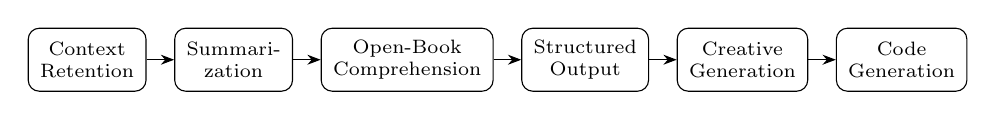
\begin{tikzpicture}[
  node distance=3.5mm,
  box/.style={draw, rounded corners, minimum height=8mm, align=center,
              font=\scriptsize, inner sep=1.5mm},
  >={Stealth[]}
]
\node[box] (c1) {Context\\Retention};
\node[box, right=of c1] (c2) {Summari-\\zation};
\node[box, right=of c2] (c3) {Open-Book\\Comprehension};
\node[box, right=of c3] (c4) {Structured\\Output};
\node[box, right=of c4] (c5) {Creative\\Generation};
\node[box, right=of c5] (c6) {Code\\Generation};
\draw[->] (c1) -- (c2);
\draw[->] (c2) -- (c3);
\draw[->] (c3) -- (c4);
\draw[->] (c4) -- (c5);
\draw[->] (c5) -- (c6);
\end{tikzpicture}
\caption{The EdgeLM capability gradient. Each family presupposes the previous:
tracking a conversation, compressing content, answering from content, obeying a
format while doing so, producing original content under constraints, and
producing executable content that transfers off Python.}
\label{fig:gradient}
\end{figure}

\subsection{Models Evaluated}
\label{sec:models}

EdgeLM evaluates fifteen openly available sub-4B models
(Table~\ref{tab:models}). The roster is deliberately not a set of independent
draws: it contains two clean base-to-finetune pairs and one within-family
post-training pair, which let us attribute differences to post-training rather
than architecture. Specifically, Hermes-3 is a full-parameter fine-tune of
Llama-3.2-3B~\cite{hermes3,llama3}; DeepScaleR-1.5B is a reinforcement-learning
fine-tune of DeepSeek-R1-Distill-1.5B~\cite{deepscaler2025,deepseekr1}; and
VibeThinker-3B is a reasoning-focused post-training of
Qwen2.5-Coder-3B~\cite{vibethinker2026,qwen25}. The roster also spans general
instruct models, reasoning-distilled models, and a community distillation
(Crow-4B, a Qwen3.5-4B model trained on Claude Opus 4.6
traces~\cite{crow4b}), giving coverage across post-training philosophies.

\begin{table}[t]
\caption{The fifteen models evaluated by EdgeLM, grouped by base family. The two
base-to-finetune pairs (Llama-3.2-3B\,$\rightarrow$\,Hermes-3 and
R1-Distill-1.5B\,$\rightarrow$\,DeepScaleR) and the within-family post-training
pair (Qwen2.5-Coder-3B\,$\rightarrow$\,VibeThinker) are highlighted in the text.}
\label{tab:models}
\centering
\footnotesize
\begin{tabular}{@{}lll@{}}
\toprule
Model & Base / lineage & Notes \\
\midrule
Qwen2.5-1.5B            & Qwen2.5            & General instruct \\
Qwen2.5-Coder-3B        & Qwen2.5-Coder      & Code-specialized base \\
Qwen3.5-4B              & Qwen3.5            & General instruct \\
VibeThinker-3B          & Qwen2.5-Coder-3B   & Reasoning post-training \\
Crow-4B                 & Qwen3.5-4B         & Opus-4.6-trace distill \\
\midrule
Llama-3.2-3B            & Llama 3.2          & General instruct (base) \\
Hermes-3-Llama-3.2-3B   & Llama-3.2-3B       & Full fine-tune; JSON/agentic \\
\midrule
DeepSeek-R1-Distill-1.5B & R1-distill (Qwen) & Reasoning distill (base) \\
DeepScaleR-1.5B         & R1-Distill-1.5B    & RL fine-tune \\
OpenReasoning-Nemotron-1.5B & Reasoning distill & Different teacher/pipeline \\
\midrule
Phi-4-mini              & Phi-4              & General instruct \\
Ministral-3B            & Mistral            & General instruct \\
SmolLM3-3B              & SmolLM3            & Multilingual reasoning \\
Gemma 3 4B              & Gemma 3            & General instruct \\
GLM-Edge-4B             & GLM-Edge           & Edge-oriented \\
\bottomrule
\end{tabular}
\end{table}

\subsection{Task Categories}
\label{sec:method}

\subsubsection{Context retention under load.}
We measure how many conversational turns a model can sustain coherent
understanding as context accumulates, rather than single-shot retrieval. A
scripted multi-turn dialogue interleaves a \emph{tracked state}---a small cast of
named entities with attributes and occasional mid-conversation updates---with
\emph{accumulating load} consisting of human-written passages on tangential
topics. At increasing turn depths we record probe accuracy (exact-match recall
or use of planted facts) and coherence (on-topic, well-formed, non-degenerate
output). The headline metric is the \emph{coherence horizon}: the turn depth and
cumulative token count at which accuracy or coherence cross a failure threshold,
together with the full degradation curve. We explicitly separate two failure
modes---context-window overflow (a capacity limit) and coherence collapse with
the relevant content still in window (a quality limit)---by logging each model's
native context window and the running token count at every turn.

\subsubsection{Cross-domain summarization.}
Each model summarizes three human-written passages---prose, mathematical, and
heavy scientific---to a fixed compression target. Summaries are scored on
faithfulness (no hallucination or contradiction; technical claims, numbers, and
logic preserved), coverage, and coherence. Faithfulness is weighted most heavily
for the mathematical and scientific passages, and is augmented by a programmatic
check that pre-extracted key claims survive in the summary. The headline metric
is the per-domain score and, crucially, the prose-to-math and prose-to-science
faithfulness drop, which operationalizes the decoupling hypothesis.

\subsubsection{Open-book comprehension.}
Each model answers graded-difficulty questions over a provided human-written
passage in three domains: literary (high-school-level prose), scientific, and
historical. Questions are tiered into literal/extractive, inferential, and
global/synthesis levels. A non-negotiable validation step ensures
\emph{answer-determinability}: every answer must follow from the passage rather
than from parametric knowledge, verified by checking whether the question can be
answered with the passage withheld. The headline metric is accuracy by domain
and difficulty tier, with the synthesis tier expected to separate models most
sharply.

\subsubsection{Structured-output compliance.}
We test adherence to explicit format contracts---valid JSON, well-formed
Markdown, code-only output, and additional custom formats---under two
conditions: format-only, and format-under-load, where the format requirement
rides on a difficult content task. Compliance is checked by deterministic
parsers and validators and is reported as a strict pass rate (exact conformance
as emitted, including the absence of prose preambles or stray code fences)
alongside a lenient rate; the gap between them characterizes failure modes. No
human reference is required for this category.

\subsubsection{Creative generation.}
Each model produces an article, a poem, and a short story under explicit
constraints (topic, length, required elements, tone, and poetic form). Scoring
separates constraint satisfaction, which is checklist-verifiable, from
qualitative quality, which is judged via position-permuted pairwise comparison
against a human-written anchor using a calibrated evaluator and a pre-registered
rubric. Because small open judges are unreliable for creative
writing~\cite{litbench2025}, this category uses a stronger judge or a retained
human-evaluation slice; the protocol is reported explicitly.

\subsubsection{Code generation.}
Each model solves a shared set of problems, each with hidden test cases, in
Python and in a low-resource language (Perl or Pascal). Using identical problems
across languages turns the task into a controlled transfer test. Scoring is
execution-based pass@1 (with optional pass@$k$), where a submission passes only
if it compiles, runs, and satisfies all hidden tests. The headline metric is
pass@1 per language and the Python-to-low-resource drop, a sharper probe of
generalization than any Python-only score.

\section{Experimental Setup}
\label{sec:setup}

Reliable comparison of small models requires care that larger-model evaluations
can often skip. We apply each model's \emph{correct} chat template, since a
mismatched template disproportionately penalizes small models and corrupts
comparisons. Quantization is pinned and reported, as it affects outputs.
Decoding is deterministic (greedy) except where sampling is intentional
(pass@$k$ and creative generation), with fixed seeds and pinned model revisions.
Where sampling is used, each item is run multiple times and reported as a mean
with confidence intervals; because human-authored item counts are modest,
confidence intervals are reported throughout. Code is executed in network-isolated
containers with CPU, memory, and wall-clock limits, and pinned interpreter and
compiler versions. Output extraction is robust for all categories except
structured-output compliance, where lenient extraction would defeat the
measurement.

Table~\ref{tab:tiers} summarizes how scoring is matched to each category. Two
categories are fully objective (deterministic parsing and code execution); two
are reliably automatable with a calibrated small-model judge; one (creative
generation) requires a stronger judge or a human slice. Stating this tiering
explicitly is itself a design choice that clarifies how much to trust each
category's automated numbers.

\begin{table}[t]
\caption{Scoring tiers. The human-authored constraint applies to stimuli; the
scorer may still be a model where validated against human judgement.}
\label{tab:tiers}
\centering
\footnotesize
\begin{tabular}{@{}lll@{}}
\toprule
Category & Primary scoring & Tier \\
\midrule
Context retention      & exact-match probe + coherence check & objective + judge \\
Summarization          & rubric judge (+ claim-survival check) & small-judge-reliable \\
Open-book comprehension & multiple-choice / short-answer & objective (mostly) \\
Structured output      & parser / validator (strict) & fully objective \\
Creative generation    & pairwise, calibrated judge / human & judge-hard \\
Code generation        & execution pass@1 & fully objective \\
\bottomrule
\end{tabular}
\end{table}

\section{Results}
\label{sec:results}

We report results for the first track of the roster: the four 1.5B models that
share (or closely share) a Qwen2.5-1.5B backbone, which together form a clean
controlled study of post-training recipes on one base. These four were executed
end-to-end through the EdgeLM harness on consumer hardware via a local Ollama
runtime, with Q4\_K\_M quantization pinned across models and the reasoning-model
decoding policy of Section~\ref{sec:setup} (sampling at $T{=}0.6$, $p{=}0.95$,
with reasoning traces split from the final answer). The remaining eleven models
in Table~\ref{tab:models} are in progress and reported as ``--'' in
Table~\ref{tab:results}; the benchmark design, stimuli, and scoring harness used
to produce every number here are contributions of this work and are shared
unchanged across the full roster. Each per-category score is a mean over the
human-authored items in that category ($n{=}5$ retention scripts, $6$
summarization passages, $18$ comprehension questions, $6$ structured-output
tasks, $6$ creative tasks, $6$ code problems).

\begin{table}[t]
\caption{Master results. Headline score per model per category, on $[0,1]$.
Ctx.\ Ret.: mean probe recall. Summ.: mean key-claim survival. Comp.: open-book
accuracy. Struct.: strict format-compliance rate. Creat.: mean
constraint-satisfaction rate (quality judged separately). Code: execution-based
pass@1 (Python executed; Perl executed; C\# static-checked). The four 1.5B-track
models are reported; the remaining eleven (``--'') are in progress.}
\label{tab:results}
\centering
\footnotesize
\setlength{\tabcolsep}{4pt}
\begin{tabular}{@{}lcccccc@{}}
\toprule
Model & Ctx.\ Ret. & Summ. & Comp. & Struct. & Creat. & Code \\
\midrule
Qwen2.5-1.5B                & \textbf{1.00} & 0.90 & 0.94 & \textbf{0.67} & \textbf{0.75} & \textbf{0.83} \\
Qwen2.5-Coder-3B            & -- & -- & -- & -- & -- & -- \\
Qwen3.5-4B                  & -- & -- & -- & -- & -- & -- \\
VibeThinker-3B              & -- & -- & -- & -- & -- & -- \\
Crow-4B                     & -- & -- & -- & -- & -- & -- \\
Llama-3.2-3B                & -- & -- & -- & -- & -- & -- \\
Hermes-3-Llama-3.2-3B       & -- & -- & -- & -- & -- & -- \\
DeepSeek-R1-Distill-1.5B    & 0.86 & 0.90 & 0.89 & 0.17 & 0.25 & 0.17 \\
DeepScaleR-1.5B             & 0.89 & 0.90 & \textbf{1.00} & 0.33 & 0.58 & 0.17 \\
OpenReasoning-Nemotron-1.5B & 0.00 & 0.73 & 0.11 & 0.17 & 0.00 & 0.00 \\
Phi-4-mini                  & -- & -- & -- & -- & -- & -- \\
Ministral-3B                & -- & -- & -- & -- & -- & -- \\
SmolLM3-3B                  & -- & -- & -- & -- & -- & -- \\
Gemma 3 4B                  & -- & -- & -- & -- & -- & -- \\
GLM-Edge-4B                 & -- & -- & -- & -- & -- & -- \\
\bottomrule
\end{tabular}
\end{table}

\subsubsection{Instruct vs.\ reasoning post-training.}
The non-reasoning control, Qwen2.5-1.5B-Instruct, is the strongest of the four on
the format- and instruction-bound categories, leading on structured output
($0.67$ strict, $0.83$ lenient), constraint satisfaction ($0.75$), and code
($0.83$ pass@1, with $3/4$ Python problems executing correctly). The
reasoning-distilled models are markedly weaker here: DeepSeek-R1-Distill-1.5B and
DeepScaleR-1.5B reach only $0.17$ and $0.33$ strict compliance and $0.17$ code
pass@1 ($0/4$ Python executed for both). Inspection of the transcripts shows the
failure is not the underlying logic but the \emph{format contract}: these models
wrap answers in long reasoning preambles and stray code fences, so an output that
contains a correct artifact still fails strict parsing---precisely the strict-vs.\
lenient gap the protocol is designed to expose. This is consistent with the
decoupling view: distillation that optimizes free-form chain-of-thought can erode
terse, format-exact emission even as it preserves reasoning content.

\subsubsection{The RL effect (DeepScaleR vs.\ R1-Distill).}
The pair DeepSeek-R1-Distill-1.5B\,$\rightarrow$\,DeepScaleR-1.5B shares a base,
so the difference between them isolates the reinforcement-learning fine-tune.
DeepScaleR improves over its base on every non-trivial category: open-book
comprehension ($0.89\!\rightarrow\!1.00$, including the synthesis tier, where it
reaches $1.00$), structured output ($0.17\!\rightarrow\!0.33$), constraint
satisfaction ($0.25\!\rightarrow\!0.58$), and context retention
($0.86\!\rightarrow\!0.89$), while code pass@1 is unchanged ($0.17$). The RL stage
thus broadens capability beyond its competition-math target without a measurable
code regression, supporting the practice of reporting lineage pairs as controlled
comparisons rather than independent leaderboard points.

\subsubsection{Truncated reasoning as a failure mode.}
OpenReasoning-Nemotron-1.5B scores near zero on retention ($0.00$),
comprehension ($0.11$), creative constraints ($0.00$), and code ($0.00$). This is
not a scoring artifact: $41$ of its $68$ logged responses ended without a closing
\texttt{</think>} tag, i.e.\ the model was still emitting its reasoning trace when
it reached the generation budget, leaving an empty final answer. The harness
records this \emph{truncated-think} state explicitly, which is what allows the
distinction between ``answered incorrectly'' and ``never produced an answer'' to
be made at all. The model retains some standalone-prompt ability---its
single-turn summarization key-claim survival is $0.73$---but the budget needed to
let it close its reasoning is far larger than its peers require at the same
quantization. This is the clearest instance in the track of the general caution
that 1.5B reasoning models consume context rapidly through accumulated traces
(Section~\ref{sec:setup}), and it argues for per-model token budgeting and for
logging the truncated-think rate as a first-class diagnostic.

\subsubsection{The decoupling signal.}
The faithfulness drop from prose to technical summarization---the direct
operationalization of the decoupling hypothesis---is small or, for the reasoning
models, reversed at this scale: the reasoning-distilled models preserve technical
key claims at least as well as prose ones (key-claim survival of
$0.7$/$1.0$/$1.0$ for prose/math/science on R1-Distill, $0.8$/$0.9$/$1.0$ on
DeepScaleR), while the instruct control is flat at $0.9$ across all three
domains. On these six passages and four models the prediction of a prose-favoring
gap is therefore not supported; if anything, reasoning post-training improves the
retention of mathematical and scientific content relative to prose. Whether this
holds across the full fifteen-model roster and a larger passage set is the
question the remainder of the benchmark is built to answer.

\section{Discussion}
\label{sec:discussion}

EdgeLM is constructed to test the reasoning--knowledge decoupling hypothesis at
the sub-4B scale. The hypothesis yields concrete, falsifiable predictions across
the gradient: models should remain competitive on code generation, structured
output, and the reasoning components of comprehension, while degrading on
knowledge-intensive open-book comprehension and faithful summarization---most
visibly in the prose-to-science faithfulness drop and the synthesis-tier
comprehension scores. The roster's two base-to-finetune pairs and one
within-family post-training pair further allow post-training effects to be
isolated from architecture: comparing a base model with its fine-tune on a fixed
backbone separates what post-training adds from what the architecture provides.
We expect these controlled comparisons to be more informative than aggregate
leaderboard positions, and we report them as first-class results.

\section{Limitations}
\label{sec:limitations}

Several limitations follow from the design. Human-authored stimuli are expensive
to produce, so per-category item counts are modest and rankings carry
non-trivial uncertainty; we mitigate this by reporting confidence intervals but
do not eliminate it. The mathematical summarization sub-domain lacks an
established human reference resource and is therefore self-curated. Reliable
automated evaluation of creative generation remains an open problem, and our
reliance on a calibrated judge or a human slice in that category is a pragmatic
compromise rather than a settled solution. Results are sensitive to quantization
and to chat-template selection; we pin and report both, but cross-study
comparison should account for them. Finally, the roster includes a community
distillation trained on another model's outputs; we report its provenance
transparently and treat its scores on equal footing with the rest of the roster,
while noting that its training pedigree differs from the openly pre-trained and
post-trained models around it.

\section{Conclusion}
\label{sec:conclusion}

We presented EdgeLM, a capability-first benchmark for sub-4B language models on
consumer hardware. In contrast to systems-first edge benchmarks that reduce task
quality to a single number, EdgeLM decomposes generative ability into six
human-authored, task-matched-scored families spanning conversational context
retention, cross-domain summarization, graded open-book comprehension,
structured-output compliance, constrained creative generation, and
execution-verified multilingual code generation. By evaluating a controlled
roster of fifteen models---including clean base-to-finetune pairs---EdgeLM is
positioned to test the reasoning--knowledge decoupling hypothesis at the scale
that on-device deployment has converged upon, and to provide a gaming-resistant,
capability-resolved complement to existing edge-LLM evaluation.

\begin{credits}
\subsubsection{\ackname} [Optional. E.g., This work was supported by \dots]

\subsubsection{\discintname}
The authors have no competing interests to declare that are relevant to the
content of this article.
\end{credits}

%
% ---- Bibliography ----
%
\bibliographystyle{splncs04}
\bibliography{references}

\end{document}
